% --------------------------------------------------------------
% This is all preamble stuff that you don't have to worry about.
% Head down to where it says "Start here"
% --------------------------------------------------------------

\documentclass[12pt]{article}

\usepackage[margin=1in]{geometry}
\usepackage{amsmath,amsthm,amssymb}
\usepackage{graphicx} %This allows to include eps figures
\usepackage{subcaption}
\usepackage[section]{placeins}
\usepackage{layout}
\usepackage{etoolbox}
\usepackage{mathabx}
\usepackage{animate}
\usepackage{array}
% This is to include code
\usepackage{listings}
\usepackage{xcolor}
\definecolor{dkgreen}{rgb}{0,0.6,0}
\definecolor{gray}{rgb}{0.5,0.5,0.5}
\definecolor{mauve}{rgb}{0.58,0,0.82}
\lstdefinestyle{Python}{
    language        = Python,
    basicstyle      = \ttfamily,
    keywordstyle    = \color{blue},
    keywordstyle    = [2] \color{teal}, % just to check that it works
    stringstyle     = \color{green},
    commentstyle    = \color{red}\ttfamily
}

\newenvironment{conditions}
  {\par\vspace{\abovedisplayskip}\noindent\begin{tabular}{>{$}l<{$} @{${}={}$} l}}
  {\end{tabular}\par\vspace{\belowdisplayskip}}

\newcommand{\N}{\mathbb{N}}
\newcommand{\Z}{\mathbb{Z}}

\newenvironment{theorem}[2][Theorem]{\begin{trivlist}
\item[\hskip \labelsep {\bfseries #1}\hskip \labelsep {\bfseries #2.}]}{\end{trivlist}}
\newenvironment{lemma}[2][Lemma]{\begin{trivlist}
\item[\hskip \labelsep {\bfseries #1}\hskip \labelsep {\bfseries #2.}]}{\end{trivlist}}
\newenvironment{exercise}[2][Exercise]{\begin{trivlist}
\item[\hskip \labelsep {\bfseries #1}\hskip \labelsep {\bfseries #2.}]}{\end{trivlist}}
\newenvironment{reflection}[2][Reflection]{\begin{trivlist}
\item[\hskip \labelsep {\bfseries #1}\hskip \labelsep {\bfseries #2.}]}{\end{trivlist}}
\newenvironment{proposition}[2][Proposition]{\begin{trivlist}
\item[\hskip \labelsep {\bfseries #1}\hskip \labelsep {\bfseries #2.}]}{\end{trivlist}}
\newenvironment{corollary}[2][Corollary]{\begin{trivlist}
\item[\hskip \labelsep {\bfseries #1}\hskip \labelsep {\bfseries #2.}]}{\end{trivlist}}



\begin{document}

% --------------------------------------------------------------
%                         Start here
% --------------------------------------------------------------

%\renewcommand{\qedsymbol}{\filledbox}

\title{Assignment 5}%replace X with the appropriate number
\author{Nalet Meinen and Pascal Wyss\\ %replace with your name
Finite Element Analysis I
}
\maketitle

\begin{figure}[!htb]
  \centering
  \vspace*{1cm}
  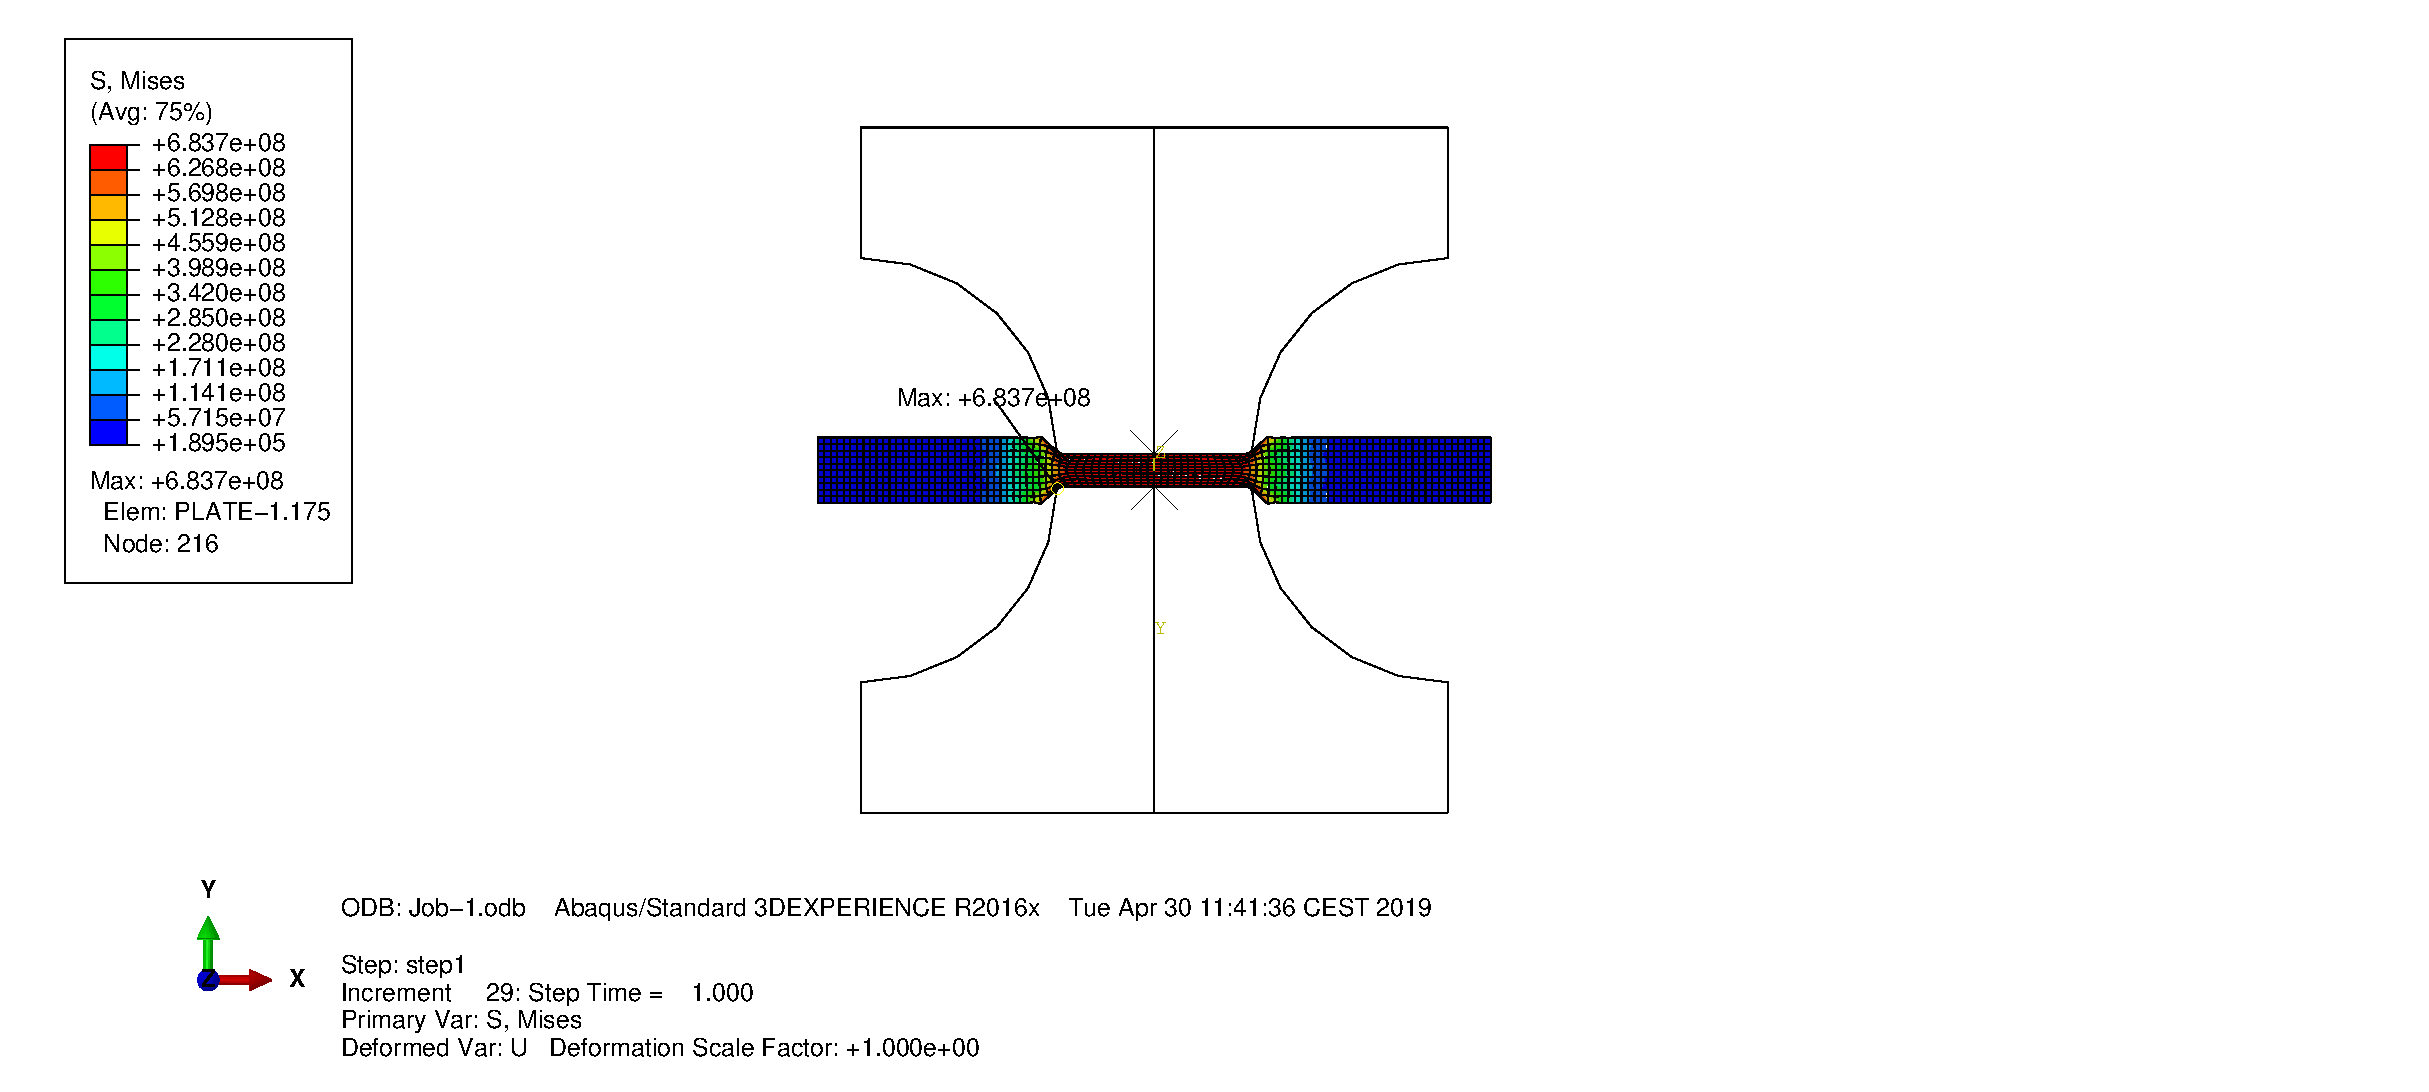
\includegraphics[trim={2cm 2cm 2cm 2cm},clip,width=1.0\linewidth]{pics/titelbild}
  \label{fig:0}
\end{figure}

\newpage

\section*{Abstract}
In this assignment, we examine the behavior of a metal plate under compression.
A rigid press, modeled as an analytical surface, squeezes the plate together.
By retrieving the force and displacement values over time, we can determine the plastic behavior of our specimen.

In this assignment, we use the findings from the previous assignment 4 and instead of using a Lagrangian 
formulation we are using a Eulerian.


% \begin{figure}[!htb]
%   \centering
%   \animategraphics[autoplay,loop,width=0.8\linewidth,trim={1mm 1mm 1mm 1mm}]{4}{pics/out/ani-}{1}{62}
%   \caption{Animation of frequency on beam}
% \end{figure}

\tableofcontents
\pagebreak
\section{Introduction}
Like in the previous assignment 4, the plate is once more compressed. Eulerian modeling can only be achieved in the 3D. As the previous model was in 2D, in this assignment we remodeled the parts in 3D once again. However, the calculations for the plasticity are the same for the material as before. Actually, the new Model is 2D alike, as we create a 2D model with a small depth so only one mesh unit is needed for the calculations. In the end, we are working with a 2D model except using the 3D Eulerian parts. 

\begin{figure}[!htb]
  \centering
  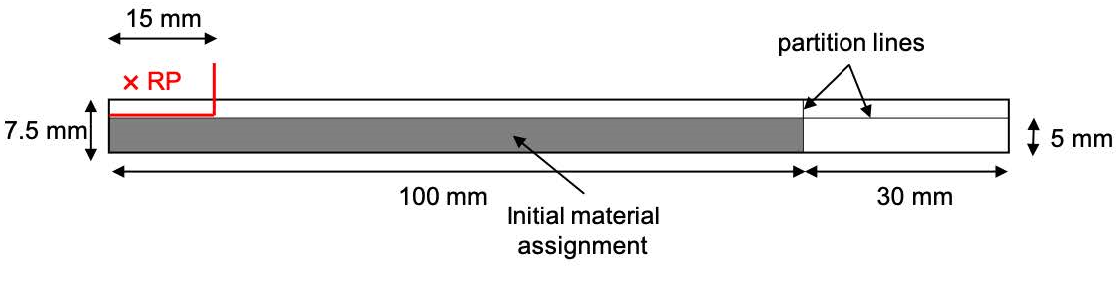
\includegraphics[width=1.0\linewidth]{pics/shematics}
  \caption{Model of the plate with Eulerian formulation}
  \label{fig:1}
\end{figure}

\noindent As shown in Figure \ref{fig:1}, the model of the plate has to be segmented. We have to set the distribution of the material, as Abaqus needs us to define where the material will be "flowing". Again, only a 4th of the model has to be sketched.

\newpage
\section{Methods}

\subsection{Coupled Lagrangian-Eulerian Analysis in Abacus}

We created a model with CPS4R mesh type. Based on the last assignments, the reduced integration
gave us the best result, so we stick with that.

\begin{figure}[!htb]
  \centering
  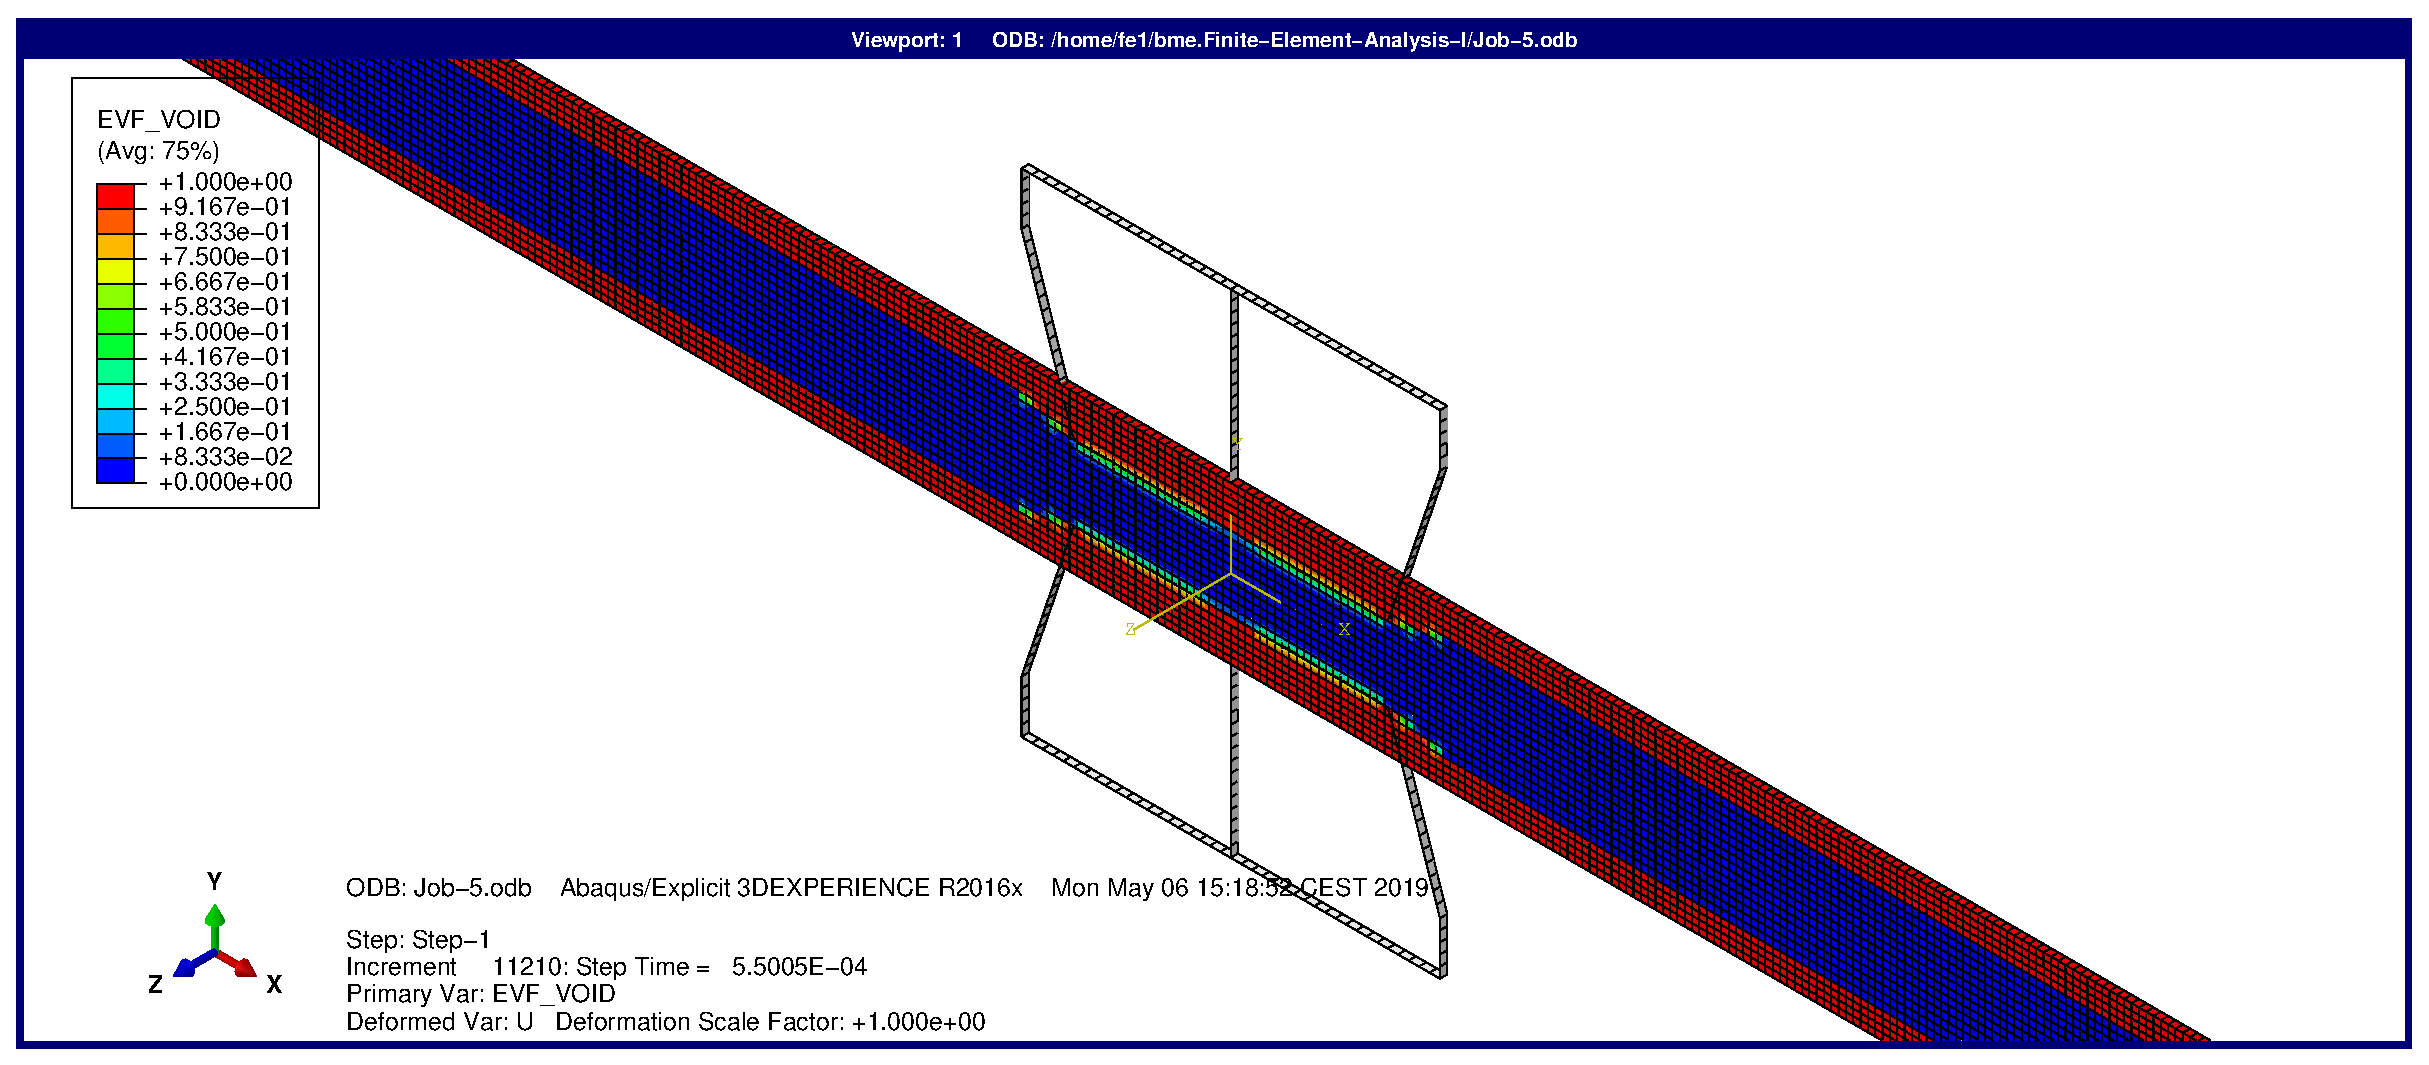
\includegraphics[width=0.9\linewidth]{pics/sexy3Dbild}
  \caption{Node to node with no sliding}
  \label{fig:2}
\end{figure}

\begin{figure}[!htb]
  \centering
  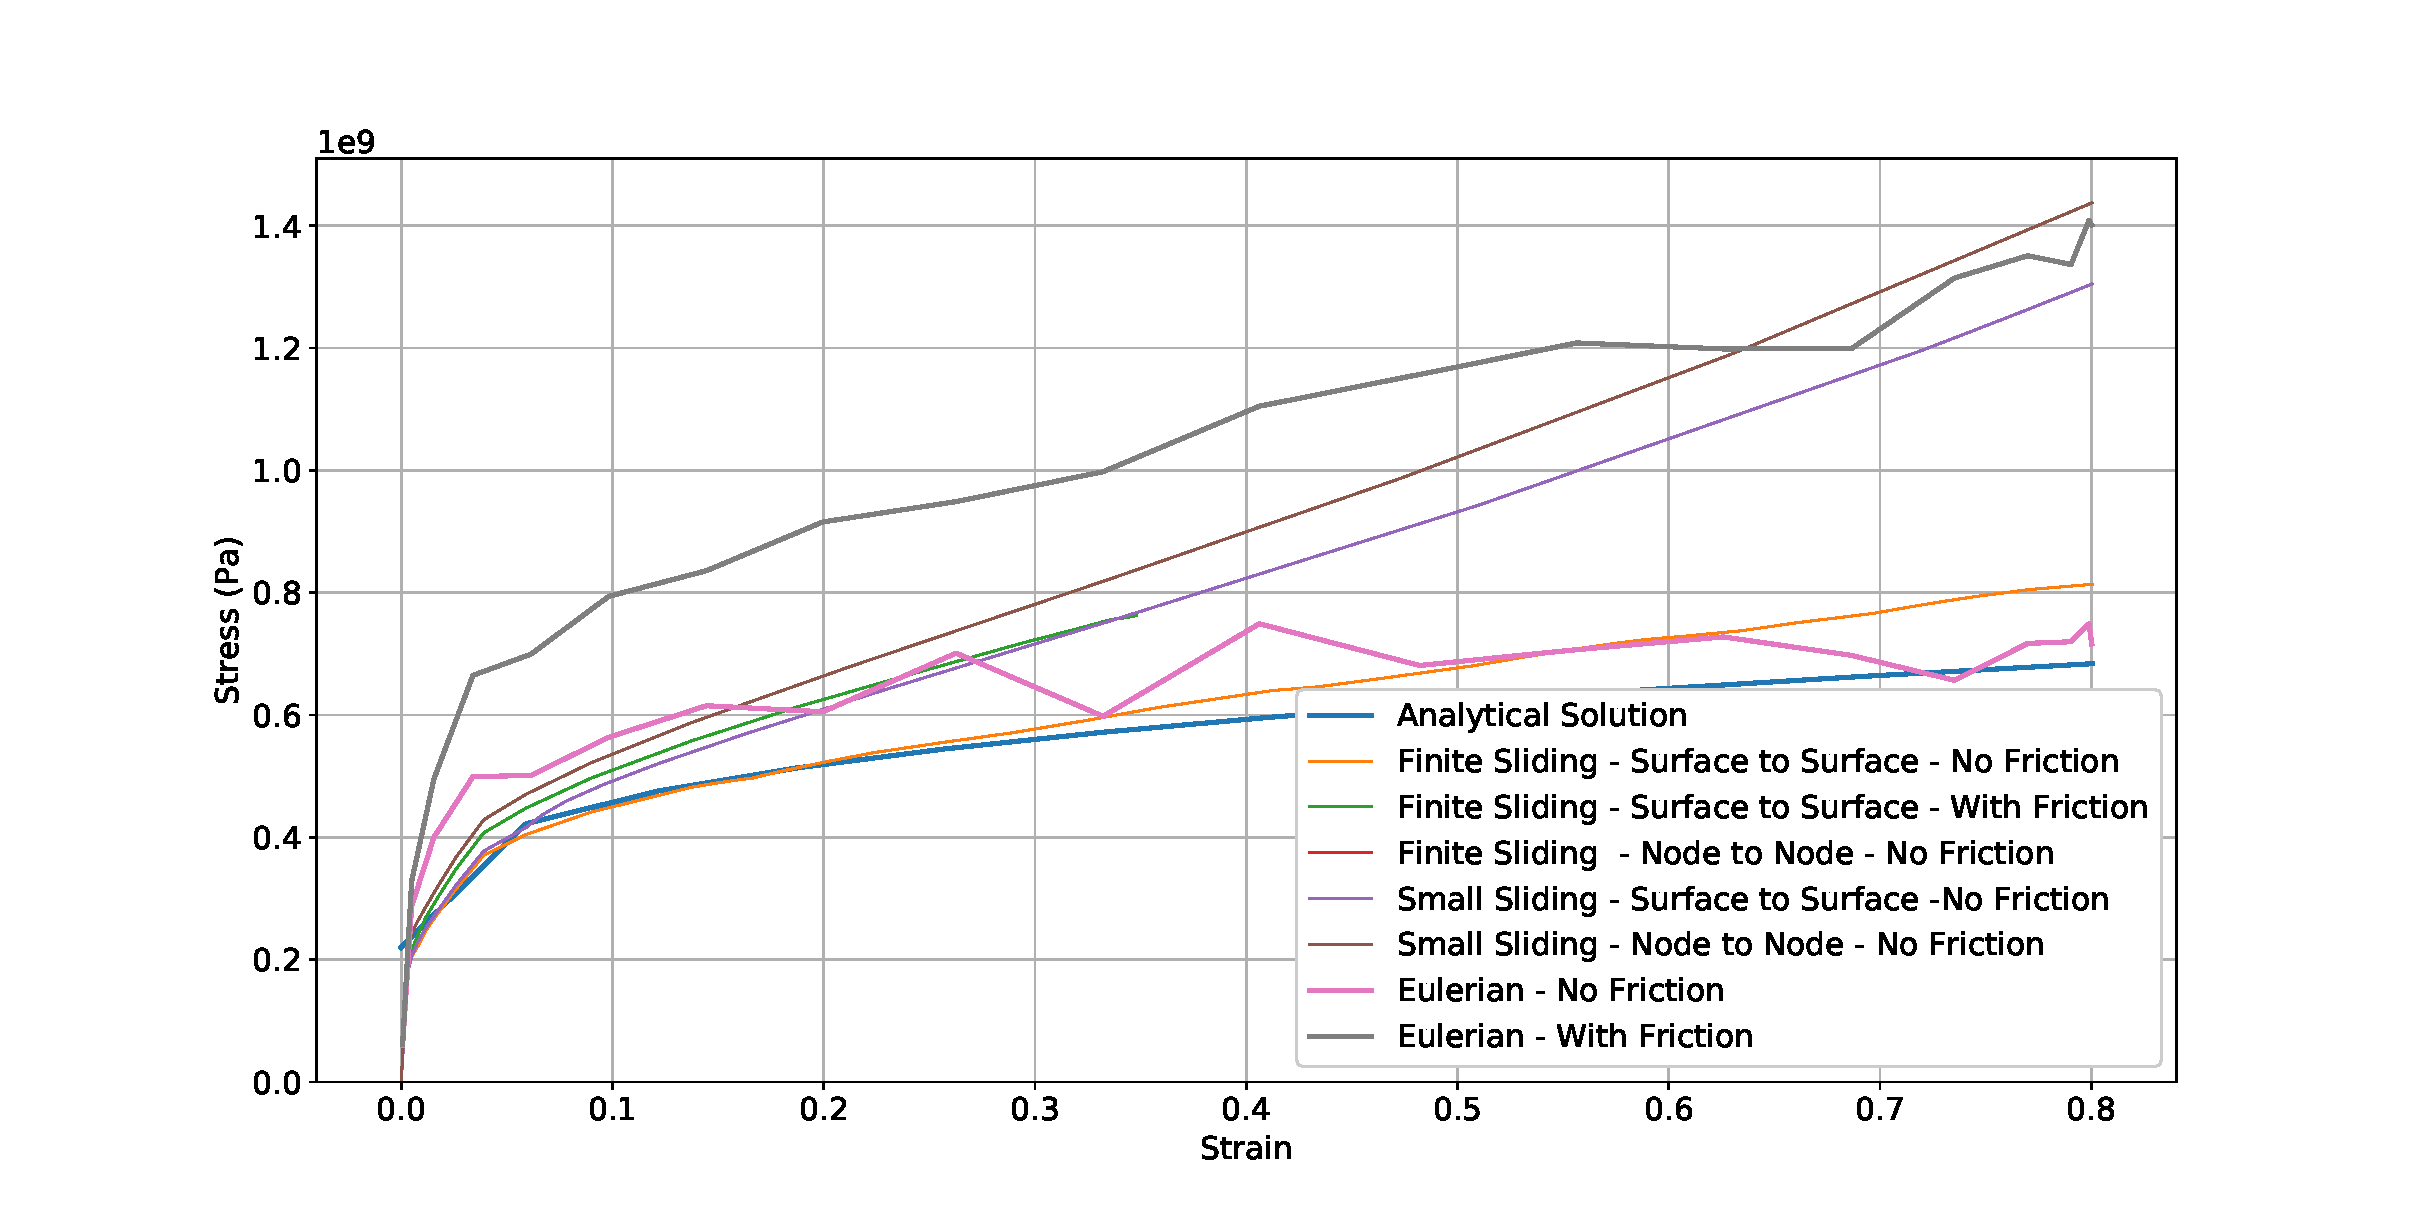
\includegraphics[width=0.9\linewidth]{pics/analytical_compared_euler}
  \caption{Result of the previous assignment with eulerian result}
  \label{fig:3}
\end{figure}


\pagebreak
\section{Results and Discussion}

The analytical and the experimental results are similar.
Logically the experiment with introduced friction (friciton coefficien 0.2) results in a higher
stress/strain ration, as energy of the compression gets lost in friction. 
during modelling, we ran into troubles with the simulation due to the sharp corner of the press.
Thus we introduced a small 1mm fillet to smoothen the process. This worked out fine and the results 
got better and were calculated more quickly.

The stress/strain ratio calculations which allowed for small sliding show a higher stress per strain ratio.


\pagebreak
\begin{thebibliography}{9}
  \bibitem{latexcompanion} 
  Michel Goossens, Frank Mittelbach, and Alexander Samarin. 
  \textit{The \LaTeX\ Companion}. 
  Addison-Wesley, Reading, Massachusetts, 1993.
\end{thebibliography}


\end{document}